\section{The Xi function, the P\'olya density and the clock}\label{ch:clock}
\label{sec:clock}

Section~\ref{ch:intro} states RH as a positivity condition on the clock $1/G$, and computation with that condition rests on four objects. The Hadamard product of $\xi$ in the variable $u=s^2$ turns RH into a statement about the zeros of an entire function of genus zero. The P\'olya kernel makes $\xi(\frac12+s)/\xi(\frac12)$ the moment generating function of a probability density, and it underlies the evaluator of Section~\ref{ch:polya}. The heat trace of the zeros turns the classes of infinitely divisible laws into sign conditions on a single function, and the explicit formula expresses it through the primes. At the basepoint $\frac12+\varepsilon$ the Thorin density is the Poisson smoothing of the zeros at every resolution $\varepsilon>0$, and it is the density of the Thorin measure of a GGC when the basepoint lies to the right of every zero; the sine squared lemma produces the same density from the primes. The rest of the book computes these objects and measures how close they come to the discrete measure that RH demands. Most of the material is classical or taken from \cite{P26}.

\subsection{The completed zeta function and the clock}

The completed zeta function $\xi$ of Section~\ref{ch:intro} is entire of order one and maximal type, satisfies $\xi(s)=\xi(1-s)$ and $\overline{\xi(\bar s)}=\xi(s)$, and is positive on the real axis. On the critical line $\Xi(\theta)=\xi(\frac12+i\theta)$ is real and even. The zeros $\rho=\beta+i\gamma$ of $\xi$ lie in the open strip $0<\re s<1$ and are symmetric under $\rho\mapsto1-\rho$ and $\rho\mapsto\bar\rho$. As in Section~\ref{ch:intro}, $G(u)=\xi(\frac12+\sqrt u)/\xi(\frac12)$, and $a_k=-(\rho_k-\frac12)^2$, one for each pair $\{\rho,1-\rho\}$.

Hadamard's theorem applied to $G$, which is entire of order $\frac12$, gives, with $u=s^2$,
\begin{equation}\label{eq:ch2:hadamard}
\frac{\xi(\frac12+s)}{\xi(\frac12)}=\prod_k\Big(1-\frac{s^2}{(\rho_k-\frac12)^2}\Big)=\prod_k\Big(1+\frac{s^2}{a_k}\Big),
\end{equation}
with $\sum|a_k|^{-1}<\infty$. Logarithmic differentiation gives the partial fraction expansion
\begin{equation}\label{eq:ch2:partial}
\frac{\xi'}{\xi}(s)=\sum_\rho\frac1{s-\rho},
\end{equation}
in which each $\rho$ is grouped with $1-\rho$, as the differentiation of \eqref{eq:ch2:hadamard} produces, or with $\bar\rho$. Grouped either way the series converges absolutely, since each group is $O(\gamma^{-2})$ for fixed $s$ and $\sum_\rho\gamma^{-2}<\infty$; without grouping it converges only when summed symmetrically in $\im\rho$. Its real part $\sum_\rho\re(s-\rho)/|s-\rho|^2$ converges absolutely without grouping.

Passing to $u=s^2$ folds each pair $\pm(\rho_k-\frac12)$ of zeros of $\xi(\frac12+s)$ into the single zero $-a_k$ of $G$, so the product has genus zero and needs no exponential factors. Since $\xi$ has no real zeros, $a_k$ is real only when $\rho_k$ lies on the critical line, and then $a_k=\gamma_k^2>0$. RH is therefore the statement that every zero of $G$ lies on the negative real axis. The reciprocal of a product of genus zero with negative zeros is a product of gamma Laplace transforms, and this is how generalised gamma convolutions enter.

A random variable $H\ge0$ is a generalised gamma convolution (GGC) if $\E e^{-uH}=\exp\{-du-\int_{(0,\infty)}\log(1+u/z)\,U(dz)\}$ for $u>0$, with a drift $d\ge0$ and a positive measure $U$, the Thorin measure, such that $\int_{(0,1)}|\log z|\,U(dz)+\int_{(1,\infty)}z^{-1}U(dz)<\infty$. The drift and the Thorin measure are unique, and the Laplace transform of a GGC extends to a holomorphic nonvanishing function on $\cut$. Section~\ref{ch:ggc} develops the class from the same definition, \eqref{eq:ch3:ggc}.

Unconditionally, $1/G$ is the Laplace transform of a probability law on $[0,\infty)$ \cite[Theorem A]{P26}; Section~\ref{ch:heat} states this as Theorem~\ref{thm:ch12:idsd} and proves it. A random variable $T$ with $\E e^{-uT}=1/G(u)$ for $u\ge0$ is called the clock variable. Its mean and variance are $\E T=\sum_ka_k^{-1}=G'(0)=\xi''(\frac12)/(2\xi(\frac12))=0.0231050$ and $\operatorname{Var}T=\sum_ka_k^{-2}=3.71726\times10^{-5}$; these constants, and $\xi(\frac12)=0.4971207781883141$, recur throughout the book. The Thorin condition asks whether $T$ is a GGC, and the answer is the rigidity theorem stated in Section~\ref{ch:intro}, which we restate with its source.

\begin{proposition}[Rigidity, {\cite[Proposition 3.4]{P26}}]\label{prop:rigid}
The clock $1/G$ is the Laplace transform of a GGC if and only if RH holds, and then its Thorin measure is $U_{\RH}$ of \eqref{eq:URH} and the clock variable is $T=\sum_{\gamma>0}e_\gamma/\gamma^2$ with independent standard exponentials $e_\gamma$.
\end{proposition}

The name refers to the absence of any freedom in the Thorin measure. If $1/G$ is the Laplace transform of a GGC with drift $d$ and Thorin measure $U$, then $d+\int U(dz)/(u+z)=G'/G(u)=\sum_k(u+a_k)^{-1}$ for $u>0$. The left side is holomorphic on $\cut$, so every pole $-a_k$ of the right side lies on the negative real axis. Hence every $a_k$ is positive, which is RH, and uniqueness of the Stieltjes representation forces $d=0$ and $U=\sum_k\delta_{a_k}$. Conversely, under RH, \eqref{eq:ch2:hadamard} writes $1/G$ as a product of gamma Laplace transforms.

\subsection{The P\'olya kernel and the P\'olya density}

Riemann's continuation of $\zeta$ writes $\xi$ as a Mellin transform of a combination of $\omega(x)=\sum_{n\ge1}e^{-\pi n^2x}$ and its derivatives, and uses the theta transformation $1+2\omega(1/x)=\sqrt x\,(1+2\omega(x))$, $x>0$. The substitution $x=e^{2u}$ turns the Mellin transform into a Fourier transform, and in Titchmarsh's normalisation \cite[Section 10.1]{Titchmarsh} the result is
\begin{equation}\label{eq:ch2:Phi}
\begin{aligned}
\Phi(u)&=2\sum_{n\ge1}\big(2\pi^2n^4e^{9u/2}-3\pi n^2e^{5u/2}\big)\exp(-\pi n^2e^{2u}),\\
\Xi(\theta)&=\int_{\mathbb R}\Phi(u)\cos(\theta u)\,du .
\end{aligned}
\end{equation}
Here $u$ is the variable of the kernel, not the argument of the clock. P\'olya studied this representation \cite{Polya}, and $\Phi$ is called the P\'olya kernel.

The kernel is even and strictly positive, and $\Phi(u)\sim4\pi^2e^{9|u|/2}\exp(-\pi e^{2|u|})$ as $|u|\to\infty$. Evenness is the functional equation read through the theta transformation (Exercise~\ref{ex:ch2:even}). For $u\ge0$ every term of \eqref{eq:ch2:Phi} is positive, because $2\pi^2n^4e^{9u/2}-3\pi n^2e^{5u/2}=\pi n^2e^{5u/2}(2\pi n^2e^{2u}-3)$ and $2\pi n^2e^{2u}\ge2\pi>3$; positivity for $u<0$ follows by evenness. Evenness also decides how $\Phi$ is computed. Term $n$ is $n^{-1/2}$ times the first term translated to the left by $\log n$, so for $u\ge0$ the first term dominates, while for $u<0$ the terms are individually of order $n^{-1/2}$ and cancel almost completely. The theta transformation turns their sum into the mirror image of the side $u>0$, and computations therefore evaluate $\Phi(|u|)$.

Each term of \eqref{eq:ch2:Phi} is entire in $u$, and since $\re e^{2u}=e^{2x}\cos2y$ for $u=x+iy$, the series converges locally uniformly in the strip $|\im u|<\pi/4$, so $\Phi$ is analytic there; the boundary lines $\im u=\pm\pi/4$ are a natural boundary inherited from the theta function \cite[Chapter 11, Section 1.4, and Chapter 5, Section 3.2]{Remmert98}. The strip of analyticity makes the trapezoid rule spectrally accurate and permits the tilted contour of Section~\ref{sec:newcomp}. Figure~\ref{fig:ch2:kernel} shows $|\Phi|$ on lines inside the strip.

\begin{figure}[htbp]
\centering
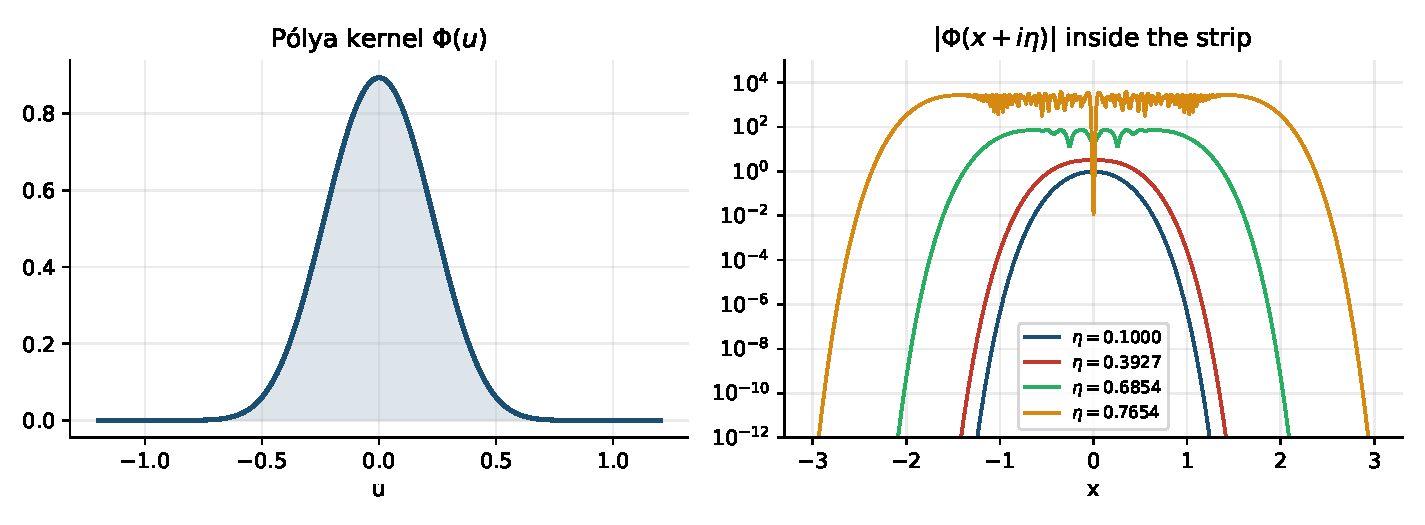
\includegraphics[width=\textwidth]{fig/kernel.pdf}
\caption{Left: the P\'olya kernel $\Phi(u)$ on the real line. Right: $|\Phi(x+i\eta)|$, on a logarithmic scale, on the lines $\eta=0.1000$, $0.3927$, $0.6854$ and $0.7654$ inside the strip of analyticity, that is at distances $0.6854$, $0.3927$, $0.1$ and $0.02$ below its edge $\eta=\pi/4$ (the tilts of Section~\ref{sec:newcomp}). As the line approaches the natural boundary $\eta=\pi/4$ the kernel grows and spreads (compare Table~\ref{tab:ch4:Meta}), and it still decays doubly exponentially in $|x|$.}
\label{fig:ch2:kernel}
\end{figure}

Since $\Xi(0)=\xi(\frac12)=\int_{\R}\Phi$, the P\'olya density $p=\Phi/\Xi(0)$ is the law of a symmetric random variable $X$ with all exponential moments, and
\begin{equation}\label{eq:ch2:mgf}
\frac{\xi(\frac12+s)}{\xi(\frac12)}=\E\,e^{sX}=\E\cosh(sX),\qquad s\in\C .
\end{equation}
The zeros of $\xi(\frac12+s)$ are therefore the complex $s$ at which the moment generating function of $X$ vanishes, and the ordinates of the zeros on the critical line are the real zeros of its characteristic function $\E\cos(\theta X)$. The clock is $1/\E\cosh(\sqrt u\,X)$, and at $u=\theta^2$ it forms with the characteristic function of $X$ a van Dantzig pair, that is, a pair $(\varphi_1,\varphi_2)$ of characteristic functions with $\varphi_2(\theta)=1/\varphi_1(i\theta)$; the name goes back to a problem of van Dantzig, which Lukacs studied \cite{Lukacs68}. Here $\varphi_1(\theta)=\Xi(\theta)/\Xi(0)$ is the characteristic function of $X$, and $1/\varphi_1(i\theta)=\xi(\frac12)/\xi(\frac12+\theta)=\E e^{-\theta^2T}$ is the characteristic function of $Z\sqrt{2T}$, with $Z$ standard normal and independent of $T$ \cite[Theorem A]{P26}. G.~Letac asked whether $\varphi_1$ is the first member of a van Dantzig pair (private communication), and Theorem~\ref{thm:ch12:idsd} shows that it is, unconditionally. Section~\ref{ch:strip} reads the reciprocal of $\xi$ along the real axis in the same way at every basepoint, and it shows by Wiener's closure theorem that the translates of $\Phi$ are not dense in $L^1(\R)$, because $\Xi$ has real zeros (Proposition~\ref{wr:prop:wiener}).

Two classical pairs show the shape to expect. The first is $(\cos\theta,1/\cosh\theta)$, the symmetric Bernoulli law on $\{-1,1\}$ with the hyperbolic secant law, and the second is $(\sin\theta/\theta,\theta/\sinh\theta)$, the uniform law on $[-1,1]$ with the logistic law scaled by $1/\pi$. In both the first member has only real zeros and the second is the product of the reciprocal factors: $1/\cosh\theta=\prod_{k\ge1}(1+\theta^2/((k-\frac12)\pi)^2)^{-1}$ is the characteristic function of $\sum_{k\ge1}L_k/((k-\frac12)\pi)$, where the $L_k$ are independent standard Laplace variables, with density $\frac12e^{-|x|}$ and characteristic function $1/(1+\theta^2)$, and likewise $\theta/\sinh\theta$ is that of $\sum_{k\ge1}L_k/(k\pi)$. The product form alone does not make a pair, since the first member must be a characteristic function in its own right, and $\prod_k(1-\theta^2/c_k^2)$ over finitely many real $c_k$ is an unbounded polynomial.

The Xi pair has the classical shape exactly when RH holds. If RH holds, $T=\sum_{\gamma>0}e_\gamma/\gamma^2$ (Proposition~\ref{prop:rigid}), and since $Z\sqrt{2e}$ is a standard Laplace variable when $e$ is a standard exponential variable independent of $Z$, $Z\sqrt{2T}$ has the law of $\sum_{\gamma>0}L_\gamma/\gamma$, the sum that Section~\ref{ch:boschA} calls $\log W$. Conversely, if $Z\sqrt{2T}$ has the law of $\sum_kL_k/c_k$ for real $c_k$ with $\sum_kc_k^{-2}<\infty$, then $\xi(\frac12+\theta)/\xi(\frac12)=\prod_k(1+\theta^2/c_k^2)$ for real $\theta$, hence for complex $\theta$, and every zero of $\xi$ lies on the critical line. Konstantopoulos, Patie and Sarkar state the same equivalence in the language of the Laguerre P\'olya class and of P\'olya frequency functions \cite[Theorem 2.3 and Corollary 2.4]{KPS24}. Table~\ref{tab:ch2:vd} computes the two members and compares them with their Hadamard products over the first $1700$ zeros, all of which lie on the line; the zeros above them enter through $\E T=\sum_ka_k^{-1}$ and $\operatorname{Var}T=\sum_ka_k^{-2}$, which are read off from the Taylor coefficients of $\log\xi(\frac12+s)$ at $s=0$ with no hypothesis on the zeros. Section~\ref{ch:strip} adds that the second member is self decomposable, that a zero off the line would contribute a factor that is not itself a characteristic function, and that away from the centre there is no such pair.

\begin{table}[htbp]
\centering\small
\begin{tabular}{rccc}
\toprule
$\theta$ & $\Xi(\theta)/\Xi(0)$ & $\xi(\frac12)/\xi(\frac12+\theta)$ & products, relative difference\\
\midrule
1 & 0.97714167 & 0.97717800 & $1\times10^{-18}$\\
2 & 0.91144824 & 0.91199057 & $8\times10^{-17}$\\
5 & 0.55429185 & 0.56739462 & $2\times10^{-14}$\\
10 & 0.076375505 & 0.11524595 & $1\times10^{-12}$\\
15 & $-1.4195704\times10^{-3}$ & $1.0310555\times10^{-2}$ & $1\times10^{-11}$\\
20 & $-7.3735457\times10^{-5}$ & $4.8509905\times10^{-4}$ & $8\times10^{-11}$\\
25 & $2.7809283\times10^{-8}$ & $1.3591692\times10^{-5}$ & $3\times10^{-10}$\\
30 & $-3.0207191\times10^{-8}$ & $2.4728825\times10^{-7}$ & $9\times10^{-10}$\\
\bottomrule
\end{tabular}
\caption{The van Dantzig pair, computed by \texttt{vdpair.py}. The last column is the larger relative difference between a member and its Hadamard product, $\prod(1-\theta^2/\gamma^2)$ or $\prod(1+\theta^2/\gamma^2)^{-1}$, over the $1700$ zeros below height $2198$, with the zeros above entering through $\sum_ka_k^{-1}$ and $\sum_ka_k^{-2}$; it is the size of the neglected term of order $\theta^6$. On $(0,30]$ the first member changes sign at $\gamma_1=14.13$, $\gamma_2=21.02$ and $\gamma_3=25.01$; the second is positive and decreasing. Both are $1-\theta^2\E T+O(\theta^4)$.}
\label{tab:ch2:vd}
\end{table}

The P\'olya variable also has a probabilistic construction. Let $S_2=\sum_{k\ge1}\frac2{\pi^2k^2}(e_k+e_k')$ with independent standard exponentials $e_k,e_k'$; it has the law of the sum of two independent hitting times of level $1$ by a three dimensional Bessel process started at $0$. By the theorem of Biane, Pitman and Yor \cite{BPY01}, going back to Williams \cite{Williams90}, $2\xi(s)=\E[(\pi S_2/2)^{s/2}]$. With $Y=\frac12\log(\pi S_2/2)$ this reads $\E e^{sY}=2\xi(s)$, so $X$ is $Y$ tilted by $e^{Y/2}$: $\E f(X)=\E[f(Y)e^{Y/2}]/\E e^{Y/2}$. Section~\ref{ch:clocklaw} uses this to estimate $\Xi$ from samples of $S_2$ and shows why sampling cannot locate the zeros. Tilting $Y$ by $e^{\alpha Y}$ in place of $e^{Y/2}$ gives, at every real basepoint $\alpha$ and with no hypothesis on the zeros, a variable $V_\alpha$ with $\E e^{sV_\alpha}=\xi(\alpha+s)/\xi(\alpha)$ and $V_{1/2}=X$ (Section~\ref{bp:sec:mellin}).

\subsection{The heat trace: spectral and arithmetic forms}

The heat trace of the zeros is
\[
W(t)=\sum_ke^{-a_kt}=\tfrac12\sum_\rho e^{(\rho-\frac12)^2t},\qquad t>0,
\]
and the series converges absolutely for every $t>0$ wherever the zeros lie, since $\re a_k=\gamma_k^2-(\beta_k-\frac12)^2>\gamma_k^2-\frac14$ for $\rho_k=\beta_k+i\gamma_k$. Integrating $e^{-(u+a_k)t}$ term by term, and using Frullani's integral $\log(1+u/a)=\int_0^\infty(1-e^{-ut})e^{-at}t^{-1}dt$ for $\re a>0$, gives, unconditionally for $u>0$ \cite[Theorem 4.3]{P26},
\[
\frac{G'}{G}(u)=\int_0^\infty e^{-ut}W(t)\,dt,\qquad \log G(u)=\int_0^\infty\big(1-e^{-ut}\big)\frac{W(t)}t\,dt .
\]
The second formula shows that $W(t)/t$ is the only possible L\'evy density of the clock variable $T$.

The classes of infinitely divisible laws of Section~\ref{sec:ch3:hierarchy} become sign conditions on $W$ \cite[Theorem 4.6]{P26}: $T$ is infinitely divisible if and only if $W\ge0$, self decomposable if and only if $W$ is nonincreasing, and a GGC if and only if $W$ is completely monotone, which by Proposition~\ref{prop:rigid} happens if and only if RH holds. The first two conditions hold unconditionally, in the strict forms $W>0$ and $W'<0$ on $(0,\infty)$ (Theorem~\ref{thm:ch12:idsd}, \cite[Theorem A]{P26}), by a proof that uses the verification of RH below height $1000$; the third is the Thorin condition, and Table~\ref{tab:ch3:hierarchy} records the rungs proved between them.

The explicit formula expresses $W$ through the primes. For even test functions $h$ holomorphic and rapidly decreasing in a strip $|\im r|\le\frac12+c$ with $c>0$, Weil's explicit formula \cite{Weil52}, \cite[Theorem 5.12]{IwaniecKowalski04}, reads
\begin{multline*}
\sum_\rho h(\gamma_\rho)=h(\tfrac i2)+h(-\tfrac i2)+\frac1{2\pi}\int_{\R}h(r)\big(\re\psi(\tfrac14+\tfrac{ir}2)-\log\pi\big)dr\\
-2\sum_{n\ge2}\frac{\Lambda(n)}{\sqrt n}\,g(\log n),
\end{multline*}
where $\rho=\frac12+i\gamma_\rho$, $g(x)=\frac1{2\pi}\int_{\R}h(r)e^{-irx}dr$ and $\psi=\Gamma'/\Gamma$ is the digamma function. The Gaussian $h(r)=e^{-r^2t}$ has $g(x)=e^{-x^2/4t}/(2\sqrt{\pi t})$ and $\sum_\rho h(\gamma_\rho)=2W(t)$, which gives the arithmetic form \cite[Theorem 4.4]{P26}
\begin{equation}\label{eq:ch2:Warith}
\begin{aligned}
W(t)&=e^{t/4}+\frac1{4\pi}\int_{\mathbb R}e^{-r^2t}m(r)\,dr-\frac1{2\sqrt{\pi t}}\sum_{n\ge2}\frac{\Lambda(n)}{\sqrt n}e^{-(\log n)^2/4t},\\
m(r)&=\re\psi\big(\tfrac14+\tfrac{ir}2\big)-\log\pi .
\end{aligned}
\end{equation}

The three terms of \eqref{eq:ch2:Warith} are the polar, archimedean and prime contributions. The polar term $e^{t/4}$ comes from $h(\pm\frac i2)$, that is, from the poles of $\pi^{-s/2}\Gamma(s/2)\zeta(s)$ at $s=1$ and $s=0$, which the factor $s(s-1)$ of $\xi$ removes. The archimedean term averages the digamma function of the gamma factor against a Gaussian and is negative for moderate $t$. The prime term is the series $\sum\Lambda(n)n^{-1/2}$ smoothed by a Gaussian of standard deviation $\sqrt{2t}$ in $\log n$: for small $t$ only the smallest primes contribute, and for large $t$ many primes contribute with nearly equal weight. As $t\to\infty$ the prime term grows like the polar term: $W(t)\to0$ and the archimedean term tends to $0$, so \eqref{eq:ch2:Warith} forces the prime term to be $e^{t/4}+o(1)$, and $W$ is what remains after the two cancel.

Table~\ref{tab:ch2:W} reproduces the comparison of \cite[Table 4.1]{P26}, and the two sides agree to fifteen digits. The polar and archimedean terms are of order one and the prime term rises from $8.4\times10^{-6}$ at $t=0.01$ to $0.30$ at $t=0.2$, while $W(t)$ decays like $e^{-\gamma_1^2t}$ with $\gamma_1^2=199.79$. An estimate of $W$ from \eqref{eq:ch2:Warith} at moderate $t$ must therefore survive a cancellation whose depth grows linearly in $t$. Section~\ref{sec:ch14:heat} extends the comparison to smaller and larger $t$ and gives that depth explicitly.

\begin{table}[htbp]
\centering\footnotesize\setlength{\tabcolsep}{4pt}
\begin{tabular}{@{}rllll@{}}
\toprule
$t$ & $W(t)$ from zeros & polar $+$ archimedean $-$ prime & archimedean & prime\\
\midrule
0.01 & 0.149698011253780 & 0.149698011253780 & $-0.8527967$ & $8.3995\times10^{-6}$\\
0.02 & $1.85412917313195\times10^{-2}$ & $1.85412917313195\times10^{-2}$ & $-0.9840612$ & 0.0024101\\
0.05 & $4.58783504857357\times10^{-5}$ & $4.58783504857357\times10^{-5}$ & $-0.9546186$ & 0.0579140\\
0.10 & $2.10479979582235\times10^{-9}$ & $2.10479979582235\times10^{-9}$ & $-0.8625096$ & 0.1628055\\
0.20 & $4.43018218022364\times10^{-18}$ & $4.43018218022364\times10^{-18}$ & $-0.7497538$ & 0.3015173\\
\bottomrule
\end{tabular}
\caption{The heat trace from the zeros and from the explicit formula, after \cite[Table 4.1]{P26}. At $t=1$ the cancellation between the arithmetic terms reaches about eighty seven digits.}
\label{tab:ch2:W}
\end{table}

\subsection{The Thorin density at a shifted basepoint}

Whether or not the Thorin condition holds at the centre, at a basepoint $\alpha$ to the right of every zero the shifted clock $u\mapsto\xi(\alpha)/\xi(\alpha+\sqrt u)$ is the Laplace transform of a GGC with an explicit Thorin density. The same formula defines a density at every basepoint $\alpha>\frac12$, whatever the zeros do, so it can be computed at every positive resolution $\alpha-\frac12$, and it is the starting point of the computations in Chapters~\ref{chap:measure} to \ref{chap:heat}. For a real basepoint $\alpha$ write $v_\alpha(r)=\re(\xi'/\xi)(\alpha+ir)$, and let $U_\alpha$ be the signed measure on $(0,\infty)$ given by
\begin{equation}\label{eq:Ualpha}
U_\alpha(dz)=\frac{v_\alpha(\sqrt z)}{2\pi\sqrt z}\,dz .
\end{equation}
At $\alpha=\frac12+\varepsilon$, where $\varepsilon>0$ is the resolution, the chart $\theta=\sqrt z$ gives $U_\alpha$ the density
\begin{equation}\label{eq:rho}
\rho_\varepsilon(\theta)=\frac1\pi\,v_{1/2+\varepsilon}(\theta)=\frac1\pi\re\frac{\xi'}{\xi}\Big(\frac12+\varepsilon+i\theta\Big),
\end{equation}
so that $U_\alpha(dz)=\rho_\varepsilon(\theta)\,d\theta$. The family $\varepsilon\mapsto\rho_\varepsilon$ is the Cauchy flow of \cite[Chapter 8]{P26}.

\begin{theorem}[{\cite[Theorem 3.7 and Remark 3.10]{P26}}]\label{thm:poisson}
If $\alpha>\re\rho$ for every zero, in particular for every $\alpha\ge1$, then $u\mapsto\xi(\alpha)/\xi(\alpha+\sqrt u)$ is the Laplace transform of a GGC $T_\alpha$ with Thorin density \eqref{eq:Ualpha}, and $v_\alpha>0$. It is the Laplace transform of a GGC if and only if $\alpha\ge\sup_\rho\re\rho$.
\end{theorem}

Since no zero lies on or to the right of the line $\re s=1$, the hypothesis of the theorem holds at $\alpha=1$, and Section~\ref{ch:basepoint} works out the shifted clock there in full. Until 2026 no smaller basepoint was known to satisfy it; the zero free half plane $\re s>\frac78$ announced in October 2026 would give every $\alpha>\frac78$ (Section~\ref{sec:ch25:open}). At every basepoint $\alpha>\frac12$ the shifted clock is still the Laplace transform of a probability law, with no hypothesis on the zeros (Theorem~\ref{bp:thm:alpha}); what the zeros decide is whether that law is a GGC. Let $P_a(x)=a/(\pi(a^2+x^2))$ denote the Poisson kernel; for $a>0$ it is the density of the Cauchy law with scale $a$, and $P_{-a}=-P_a$. Write $\mu_\varepsilon$ for the signed measure $U_{1/2+\varepsilon}$, and use the same symbol for its image in the chart $\theta=\sqrt z$, where it has the density \eqref{eq:rho}. By Theorem~\ref{thm:poisson}, $\mu_\varepsilon$ is the Thorin measure of the GGC $T_{1/2+\varepsilon}$ when $\frac12+\varepsilon>\re\rho$ for every zero, in particular for every $\varepsilon\ge\frac12$, and we call it the Thorin measure at resolution $\varepsilon$ in general. Grouping each zero with its partners under $\rho\mapsto1-\bar\rho$ and $\rho\mapsto\bar\rho$ gives the unconditional structure of its density.

\begin{proposition}[Poisson structure]\label{prop:struct}
For $\varepsilon>0$ and $\theta\ge0$ such that $\frac12+\varepsilon+i\theta$ is not a zero of $\xi$,
\begin{multline}\label{eq:struct}
\rho_\varepsilon(\theta)=\sum_{\gamma>0,\ \re\rho=1/2}\big[P_\varepsilon(\theta-\gamma)+P_\varepsilon(\theta+\gamma)\big]\\
+\sum_{\text{off line }\rho=\frac12\pm\delta+i\gamma,\ \gamma>0}\Big(\big[P_{\varepsilon+\delta}+P_{\varepsilon-\delta}\big](\theta-\gamma)+\big[P_{\varepsilon+\delta}+P_{\varepsilon-\delta}\big](\theta+\gamma)\Big),
\end{multline}
where the second sum counts each off line pair $\{\frac12+\delta+i\gamma,\frac12-\delta+i\gamma\}$, $0<\delta<\frac12$, once. Equivalently, with $\alpha=\frac12+\varepsilon$, $\rho_\varepsilon(\theta)$ is the sum of $P_{\alpha-\beta}(\theta-\gamma)+P_{\alpha-\beta}(\theta+\gamma)$ over the zeros $\rho=\beta+i\gamma$ with $\gamma>0$. In particular, under RH, $\mu_\varepsilon=P_\varepsilon*U^{\pm}_{\RH}$ restricted to $\theta>0$, where $U^\pm_{\RH}=\sum_{\gamma>0}(\delta_\gamma+\delta_{-\gamma})$.
\end{proposition}

\begin{proof}
Take real parts in \eqref{eq:ch2:partial} at $s=\alpha+i\theta$ with $\alpha=\tfrac12+\varepsilon$: a zero $\rho=\beta+i\gamma$ contributes $\pi P_{\alpha-\beta}(\theta-\gamma)$ to $v_\alpha(\theta)$, and $\alpha-\beta=\varepsilon\mp\delta$ when $\beta=\frac12\pm\delta$. Dividing by $\pi$ and grouping each zero $\rho$ with $\bar\rho$ gives the second form, and collecting the zeros $\rho$, $\bar\rho$, $1-\rho$ and $1-\bar\rho$ gives \eqref{eq:struct}. The series converges absolutely, and uniformly for $\theta$ in compact sets avoiding the zeros, since each term is $O(\gamma^{-2})$ there and $\sum_\rho\gamma^{-2}<\infty$.
\end{proof}

Each zero on the line thus contributes a Poisson kernel of width $\varepsilon$ centred at its ordinate, and a small reflected kernel centred at minus the ordinate. An off line pair contributes kernels of widths $\varepsilon+\delta$ and $\varepsilon-\delta$, and the second is negative once $\varepsilon<\delta$, that is, once the line $\re s=\frac12+\varepsilon$ lies to the left of the zero $\frac12+\delta+i\gamma$. If every zero lies to the left of the line, every kernel is positive and so is $v_\alpha$; a negative value of $v_\alpha$ therefore proves a zero to the right of $\alpha$.

\begin{remark}[Positivity on one line]\label{rem:ch2:oneline}
The criterion of Theorem~\ref{thm:poisson} concerns the analytic continuation of the shifted clock, not the sign of $v_\alpha$ on the single line $\re s=\alpha$. Once a zero $\rho$ lies to the right of the line, the shifted clock ceases to be a GGC, since $\xi(\alpha+\sqrt u)$ vanishes at $u=(\rho-\alpha)^2\in\cut$, but the density need not change sign, because the positive kernels of the other zeros can outweigh the negative one. Exercise~\ref{ex:ch2:line} gives an entire function with the order, symmetry and reality of $\xi$ whose density is positive on a line with a zero to its right; for $\xi$ itself it is not known, without assuming RH, whether positivity on one line excludes zeros to its right. Section~\ref{sec:ch13:visibility} gives, to first order in $\varepsilon$, the condition under which an off line zero makes $\rho_\varepsilon$ negative at its ordinate, and Section~\ref{ch:almost} bounds the negative part of $\mu_\varepsilon$ with no hypothesis, through zero density estimates. Positivity on every line to the right of $\re s=\sigma_0$ does exclude zeros there: if $v_\alpha\ge0$ for every $\alpha>\sigma_0$, then no zero has $\re\rho>\sigma_0$, because $\re(\xi'/\xi)(\rho-b)\sim-m/b$ as $b\downarrow0$ at a zero $\rho$ of multiplicity $m$. With $\sigma_0=\frac12$ this is Lagarias's criterion \cite{Lagarias}: RH holds if and only if $v_\alpha\ge0$ for every $\alpha>\frac12$.
\end{remark}

Integrated over $\theta>0$, a line zero contributes mass one, which concentrates at $\theta=\gamma$ as $\varepsilon\downarrow0$. An off line pair contributes mass two when $\varepsilon>\delta$, and when $\varepsilon<\delta$ a signed measure of mass zero whose total variation tends to zero as $\varepsilon\downarrow0$. These limits can be summed over the zeros: if $f$ is continuous with support in $[a,b]\subset(0,\infty)$, then for $0<\varepsilon\le1$ each term of \eqref{eq:struct} with $\gamma>b+1$ integrates $f$ to a number of modulus at most $C_f\gamma^{-2}$, where $C_f$ depends only on $f$, because the widths $c$ in \eqref{eq:struct} satisfy $|c|<\varepsilon+\frac12\le\frac32$, $|P_c(x)|\le|c|/(\pi x^2)$, and $|\theta\pm\gamma|\ge\gamma-b\ge\gamma/(b+1)$ for $\theta\in[a,b]$; as $\sum_\rho\gamma^{-2}<\infty$, dominated convergence applies to the sum over the zeros. Hence $\mu_\varepsilon\to U_{\rm line}=\sum_{\text{line zeros}}\delta_{\gamma^2}$ vaguely, whatever the truth of RH \cite[Proposition 9.5]{P17}. Sections~\ref{ch:distances}, \ref{ch:offline}, \ref{ch:turing}, \ref{ch:weak} and \ref{ch:deconv} build on this description.

\subsection{The sine squared lemma: the Thorin density from the primes}

The sine squared lemma produces the same Thorin density from the L\'evy side, where the primes appear as atoms. For $x>0$ and $s\ge0$,
\begin{equation}\label{eq:sin2}
e^{-sx}+sx-1=x\int_0^\infty\log\Big(1+\frac{s^2}{z}\Big)\frac{\sin^2(x\sqrt z/2)}{\pi\sqrt z}\,dz .
\end{equation}
To prove it, substitute $z=\theta^2$, which turns the right side into $\frac x\pi\int_0^\infty\log(1+s^2/\theta^2)(1-\cos x\theta)\,d\theta$. Both sides vanish at $s=0$, and their derivatives in $s$ agree because $\int_0^\infty(1-\cos x\theta)\,2s(\theta^2+s^2)^{-1}d\theta=\pi(1-e^{-sx})$. Thus a single compensated exponential $e^{-sx}+sx-1$, the compensated Laplace exponent of one jump of size $x$, is a positive superposition of the logarithms $\log(1+s^2/z)$ that define Thorin measures in the variable $s^2$. The weight $\sin^2(x\sqrt z/2)$ vanishes when $\sqrt z$ is a multiple of $2\pi/x$ and oscillates with that period, so a jump at $x=\log n$ becomes an oscillation in $\sqrt z$ with frequency $\log n$. This is how the prime atoms of the explicit formula turn into the oscillating Thorin density of the reciprocal.

\begin{remark}[A first passage proof]\label{rem:dbeta:ig}
The original proof of \eqref{eq:sin2} \cite[Lemma 8.1]{P17}, as recalled in \cite{P26beta}, goes through the first passage time $\tau_x$ of a standard Brownian motion to the level $x>0$, which has the density $x(2\pi t^3)^{-1/2}e^{-x^2/(2t)}$ and the Laplace transform $\E e^{-s^2\tau_x/2}=e^{-sx}$. As $x\mapsto\tau_x$ is a positive stable subordinator of index one half with L\'evy density $(2\pi t^3)^{-1/2}$, also $\int_0^\infty(1-e^{-s^2t/2})(2\pi t^3)^{-1/2}\,dt=s$, and the three facts combine into
\begin{equation}\label{eq:dbeta:ig}
e^{-sx}+sx-1=\int_0^\infty\big(1-e^{-s^2t/2}\big)\big(1-e^{-x^2/(2t)}\big)\frac{x\,dt}{\sqrt{2\pi t^3}},\qquad s,x>0,
\end{equation}
an integral of a positive function. By the Fourier transform of the Gaussian, $1-e^{-x^2/(2t)}=2\int_0^\infty(1-\cos x\theta)\sqrt{t/(2\pi)}\,e^{-t\theta^2/2}\,d\theta$. Substituting this, exchanging the integrals, which Tonelli's theorem allows, and using Frullani's integral $\int_0^\infty\big(e^{-t\theta^2/2}-e^{-t(\theta^2+s^2)/2}\big)\,dt/t=\log(1+s^2/\theta^2)$ gives
\[
e^{-sx}+sx-1=\frac x\pi\int_0^\infty\log\Big(1+\frac{s^2}{\theta^2}\Big)(1-\cos x\theta)\,d\theta,
\]
which is \eqref{eq:sin2} in the variable $\theta=\sqrt z$. In this proof the jump size $x$ enters only through the factor $1-e^{-x^2/(2t)}$, whose Gaussian Fourier transform produces the weight $1-\cos x\theta=2\sin^2(x\theta/2)$, and the Laplace variable only through the factor $1-e^{-s^2t/2}$, which Frullani's integral turns into the logarithm. The script \texttt{dbeta\_thorin.py} evaluates both sides of \eqref{eq:dbeta:ig} at $s=1.3$ and $x=0.8$, where they agree in all fourteen digits printed, $0.39345468195878$.
\end{remark}

Integrating \eqref{eq:sin2} against a measure turns L\'evy representations into Thorin representations. A L\'evy representation $\log f(\alpha+s)/f(\alpha)=cs+\int(e^{-sx}+sx-1)L(dx)$ for $s\ge0$, with $c$ real and $L$ a real measure on $(0,\infty)$ such that $\int\min(x,x^2)\,|L|(dx)<\infty$, becomes a Thorin representation with density $(2\pi\sqrt z)^{-1}[c+\int2\sin^2(x\sqrt z/2)\,xL(dx)]$, and the bracket equals $\re(f'/f)(\alpha+i\sqrt z)$ \cite[Theorem 8.2]{P17}. For $f=\xi$ at $\alpha>1$ the input is the signed canonical measure $xL(dx)$, with atoms $\Lambda(n)n^{-\alpha}$ at $\log n$, an archimedean density and a pole density \cite[Theorem 8.1]{P26}.

Table~\ref{tab:prime} compares the two routes: the bracket computed from the canonical measure with the primes truncated at $N=2\times10^6$, and $v_\alpha(\theta)$ computed by the P\'olya route of Section~\ref{ch:polya}. At $\alpha=1.5$ and $\alpha=2$ the difference is the prime tail $\sum_{n>N}\Lambda(n)n^{-\alpha}(1-\cos(\theta\log n))$, of order $N^{1-\alpha}/(\alpha-1)$, that is $1.4\times10^{-3}$ and $5\times10^{-7}$. At $\alpha=3$ the tail is of order $10^{-13}$, the error in the row $\theta=14.1347$, and the larger discrepancy at $\theta=50$ comes from the double precision quadrature of the archimedean integral, not from the primes. The P\'olya values carry only the spectrally small discretisation error of the trapezoid rule.

\begin{table}[t]
\centering\small
\begin{tabular}{rrlll}
\toprule
$\alpha$ & $\theta$ & sine squared, primes $\le 2\times10^6$ & P\'olya route & error of prime side\\
\midrule
3.0 & 14.1347 & 0.561447238789 & 0.561447238789 & $1.1\times10^{-13}$\\
3.0 & 50 & 1.120967014740 & 1.120967015289 & $5.5\times10^{-10}$\\
2.0 & 14.1347 & 0.766398694727 & 0.766399169607 & $4.7\times10^{-7}$\\
2.0 & 50 & 1.224475714058 & 1.224476216908 & $5.0\times10^{-7}$\\
1.5 & 14.1347 & 1.065762504228 & 1.067140080666 & $1.4\times10^{-3}$\\
1.5 & 50 & 1.385288214458 & 1.386706213218 & $1.4\times10^{-3}$\\
\bottomrule
\end{tabular}
\caption{The bracket $v_\alpha(\theta)$ of the sine squared lemma computed from the canonical measure (drift, archimedean integral, pole term and primes up to $2\times10^6$) and from the P\'olya density; $\theta=14.1347$ is the first ordinate $\gamma_1$, rounded. The P\'olya values agree with an independent evaluation of $\re(\xi'/\xi)$ through $\Gamma$ and $\zeta$ to about $10^{-15}$.}
\label{tab:prime}
\end{table}

Three continuations enter the book and should be kept apart \cite[Section 3.3]{P26}. Riemann's continuation of $\zeta$ by the theta transformation makes $\xi$ entire, and the P\'olya representation \eqref{eq:ch2:Phi} is this continuation in Fourier form. The continuation of the Laplace transform $\E e^{-uT}$ from $u\ge0$ to the meromorphic function $1/G$ uses no arithmetic; it gives the L\'evy form of the clock and places the atoms of the Thorin measure at the points $a_k$. The series $-\zeta'/\zeta(s)=\sum\Lambda(n)n^{-s}$ converges absolutely only for $\re s>1$, and although each of its terms is entire the sum is not; the explicit formula reaches the critical line only after the terms are paired with a test function whose transform decays, as in \eqref{eq:ch2:Warith}. The difference between continuing the terms and continuing the sum reappears in Section~\ref{ch:sin2more} as the cost of computing from the primes.
